\section{Experiments}
\label{sec:exp}

\blue{Section~\ref{sec:exp_main} gives the setup. Sections~\ref{sec:exp_results} and~\ref{sec:exp_efficiency} compare \sysname and \sysLA with the baselines in accuracy and cost, and Section~\ref{sec:exp_ablation} analyzes the components of \sysname. Section~\ref{sec:exp_theory} then tests the theory of Section~\ref{sec:theory} on trained checkpoints, and Section~\ref{sec:exp_ladder} attributes the gains of \sysLA to its two components.}

\subsection{\blue{Setup}}
\label{sec:exp_main}

\blue{The code is available at} \url{\codeurl}.

\fakeparagraph{Datasets and Setup}
Experiments are performed on seven widely used long-term time series forecasting datasets: 
\textit{ETTh1}, 
\textit{ETTh2}, 
\textit{ETTm1}, 
\textit{ETTm2}\footnote{\url{https://github.com/zhouhaoyi/ETDataset}}, 
\textit{Weather}\footnote{\url{https://www.bgc-jena.mpg.de/wetter/}}, 
\textit{Electricity}\footnote{\url{https://archive.ics.uci.edu/ml/datasets}}, 
and \textit{Traffic}\footnote{\url{https://pems.dot.ca.gov/}}, 
covering a diverse range of real-world scenarios.
The details of the datasets are provided in \blue{the electronic supplement}.
Following prior works~\citep{nie2023patchtst, zhang2023crossformer, huang2025timebase}, we adopt a 6:2:2 split for the ETT datasets and a 7:1:2 split for the other datasets. 
For \sysname, we report the average results over three random seeds, while for the other baselines we follow their official implementations and released code. 
We evaluate the forecasting \textbf{accuracy} of all tested models using mean squared error (MSE) and mean absolute error (MAE), 
and assess \textbf{efficiency} in terms of floating-point operations (FLOPs) and the number of parameters (Params).

\fakeparagraph{Baselines and Implementation Details}
% We evaluate our approach against eight competitive baselines, encompassing both state-of-the-art Transformer architectures and parameter-efficient forecasting models.  
\revised{
We evaluate our approach against eight competitive baselines, following the standard non-pretraining setting where all models are trained and evaluated directly on domain-specific datasets. 
The baselines span both state-of-the-art Transformer-based architectures and recent parameter-efficient forecasting models.
}
We compare our method with PatchTST \citeyearpar{nie2023patchtst}, iTransformer \citeyearpar{liu2023itransformer}, Crossformer \citeyearpar{zhang2023crossformer}, FEDformer \citeyearpar{zhou2022fedformer}, TimeBase \citeyearpar{huang2025timebase}, SparseTSF \citeyearpar{lin2024sparsetsf}, FITS \citeyearpar{fits2024}, and TimeMixer \citeyearpar{timemixer24}.
Among these, PatchTST, Crossformer, and TimeMixer are patch-based; SparseTSF is phase-based; TimeBase integrates patch and phase paradigms; FITS and FEDformer are frequency-domain; and iTransformer models the full sequence directly.
For all baselines, we adopt the recommended configurations provided in their official implementations\revised{, keeping hyperparameters aligned with ~\cite{huang2025timebase}.}
The model is optimized using the Adam optimizer with a fixed learning rate of $1 \times 10^{-3}$.  
Following the settings from efficiency-oriented works~\citep{huang2025timebase, lin2024sparsetsf, fits2024}, the look-back length is set to 720 time steps.
More implementation details are provided in \blue{the electronic supplement}.

\blue{
\fakeparagraph{Setup for \sysLA}
\label{sec:ext_setup}
\sysLA uses the \sysname backbone of each setting (a setting is one dataset with one horizon, 28 in total) with the components of Section~\ref{sec:extension}. It is trained from scratch with the Huber loss, at most 30 epochs with early stopping on the validation loss (patience 8), with three seeds (2021--2023). The Huber loss is chosen for its linear tail, which keeps sharp level shifts from dominating the gradient and stabilizes training. All runs of \sysL and \sysLA use the input length $L=720$, the period $P=24$, and the seven datasets and four horizons above. \sysL and \sysLA are built from the same random state for each setting and seed, so that they produce identical forecasts at initialization whenever they share the gate initialization (Section~\ref{sec:ext_init}). On the settings that keep the default extension hyperparameters, their differences are therefore due to the modulation alone; on the eight settings where the per-setting search below changed these hyperparameters for \sysLA only, the differences also reflect those changes.

Before the 28-setting runs, we fixed the remaining design choices on the validation split of one setting per dataset (ETTh1-96, ETTh2-720, ETTm1-336, ETTm2-96, Weather-192, Electricity-96 and Traffic-96). The branch decoder was chosen among three variants of the same rank: learned decoders on 30 or 90 pooled values, and the fixed displacement, tilt and curvature profiles of \equref{eq:branch}. The gates were chosen per dataset between per-channel and shared. The rule preferred the variant with the fewest parameters whenever the validation errors were within 0.5\%, and it selected shared gates when they were within 0.1\% of per-channel gates. It selected the fixed profiles for every dataset, and shared gates for ETTh2, ETTm1 and ETTm2. The remaining hyperparameters of the extension --- the modulation width $w$, the learning-rate multiplier of the extension parameters, and the gate initialization --- were selected per setting by a small grid search on the five datasets other than ETTh1 and ETTh2, whose settings keep the default values.

We report \sysLA in two configurations. The \emph{main-table configuration} of Table~\ref{tab:main_results} is the per-setting-tuned deployment configuration: it extends the per-setting search to further extension hyperparameters, including the basis of the level branch and whether the modulation is active at inference, which the search switches off on five settings (Appendix~\ref{app:la_config}). The \emph{protocol configuration} keeps one branch design, the fixed profiles, on every setting and the modulation always active at inference, so that the mechanism analyses of Sections~\ref{sec:exp_theory} and~\ref{sec:exp_ladder} are defined in the same way on all 28 settings; it is the instrument of these controlled attributions rather than a deployment recipe. Those sections compare it with \sysL and with the \sysname backbone retrained under the same protocol, which we call \sysname (retrained), as opposed to \sysname (conference), the result of the conference version. The dataset averages of the two \sysLA configurations differ by between 0.3\% and 2\%.
}

\subsection{\blue{Main Results}}
\label{sec:exp_results}

We conduct a joint evaluation of model efficiency and predictive accuracy. 
The comparative analysis highlights that the proposed \textit{\sysname} establishes an improved effectiveness-efficiency tradeoff in terms of parameter scale and error metrics.

\begin{table*}[t]
\centering
\caption{
Main results for long-term forecasting.
\blue{The input length is $L=720$, and results are averaged over the horizons $H\in\{96,192,336,720\}$.}
The best results are shown in \best{bold}, and the second-best in \second{underline}.
\blue{The \sysname row is \sysname (conference). \sysLA uses the main-table configuration (Section~\ref{sec:ext_setup}) and is averaged over three seeds; bold and underline marks are assigned among the baselines and \sysname only, so the \sysLA row is reported as a reference and carries no marks by design, even where it is the best entry.}
}
\label{tab:main_results}
\footnotesize
\setlength{\tabcolsep}{3.6pt}
\begin{tabular}{l|cc|cc|cc|cc|cc|cc|cc}
\hline
\multirow{2}{*}{Model}
& \multicolumn{2}{c|}{ETTh1}
& \multicolumn{2}{c|}{ETTh2}
& \multicolumn{2}{c|}{ETTm1}
& \multicolumn{2}{c|}{ETTm2}
& \multicolumn{2}{c|}{Electricity}
& \multicolumn{2}{c|}{Traffic}
& \multicolumn{2}{c}{Weather} \\
\cline{2-15}
 & MSE & MAE & MSE & MAE & MSE & MAE & MSE & MAE & MSE & MAE & MSE & MAE & MSE & MAE \\
\hline
\blue{\sysLA} & \blue{0.401} & \blue{0.418} & \blue{0.341} & \blue{0.387} & \blue{0.351} & \blue{0.379} & \blue{0.248} & \blue{0.313} & \blue{0.159} & \blue{0.250} & \blue{0.392} & \blue{0.252} & \blue{0.219} & \blue{0.256} \\
\hline
\sysname & \best{0.403} & \best{0.415} & 0.346 & 0.388 & \best{0.346} & \best{0.374} & \best{0.250} & \best{0.313} & \best{0.160} & \best{0.250} & \best{0.386} & \best{0.249} & \best{0.223} & \best{0.260} \\
PatchTST & 0.420 & 0.439 & \second{0.344} & 0.390 & \second{0.354} & 0.383 & 0.251 & 0.319 & 0.169 & 0.265 & \second{0.394} & \second{0.266} & \second{0.223} & 0.264 \\
iTransformer & 0.453 & 0.467 & 0.392 & 0.422 & 0.370 & 0.401 & 0.278 & 0.337 & \second{0.165} & 0.263 & 0.406 & 0.290 & 0.233 & 0.273 \\
Crossformer & 0.517 & 0.512 & 1.468 & 0.867 & 0.390 & 0.417 & 0.392 & 0.426 & 0.180 & 0.273 & 0.545 & 0.282 & 0.255 & 0.304 \\
FEDformer & 0.523 & 0.523 & 0.428 & 0.469 & 0.438 & 0.465 & 0.401 & 0.452 & 0.235 & 0.348 & 0.638 & 0.400 & 0.354 & 0.393 \\
TimeBase & \second{0.404} & \second{0.416} & 0.347 & 0.397 & 0.356 & \second{0.380} & \best{0.250} & \second{0.314} & 0.167 & \second{0.258} & 0.418 & 0.278 & 0.227 & \second{0.262} \\
SparseTSF & 0.406 & 0.418 & 0.345 & \second{0.383} & 0.362 & 0.383 & 0.252 & 0.316 & 0.168 & 0.263 & 0.413 & 0.280 & 0.243 & 0.285 \\
FITS & 0.419 & 0.435 & \best{0.334} & \best{0.382} & 0.359 & 0.382 & 0.285 & 0.336 & 0.172 & 0.270 & 0.410 & 0.290 & 0.241 & 0.283 \\
TimeMixer & 0.452 & 0.474 & 0.386 & 0.425 & 0.383 & 0.413 & 0.314 & 0.367 & 0.171 & 0.273 & 0.421 & 0.298 & 0.237 & 0.281 \\
\hline
\end{tabular}
\end{table*}

\begin{figure*}[t]
    \centering
    % 子图1 - Traffic FLOPs
    \begin{subfigure}{0.24\textwidth}
        \centering
        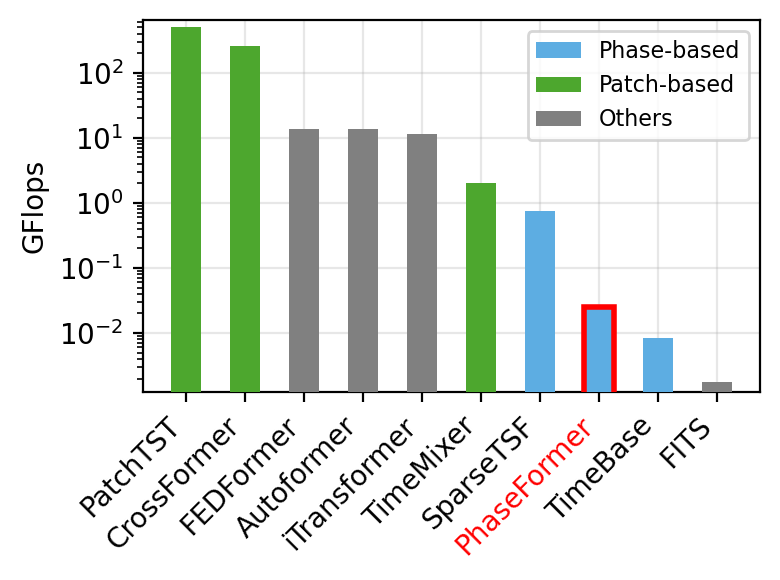
\includegraphics[width=\linewidth]{figures/flops_traffic.png}
        \caption{FLOPs on Traffic}
        \label{fig:traffic_flops}
    \end{subfigure}
    % 子图2 - Traffic Params
    \begin{subfigure}{0.24\textwidth}
        \centering
        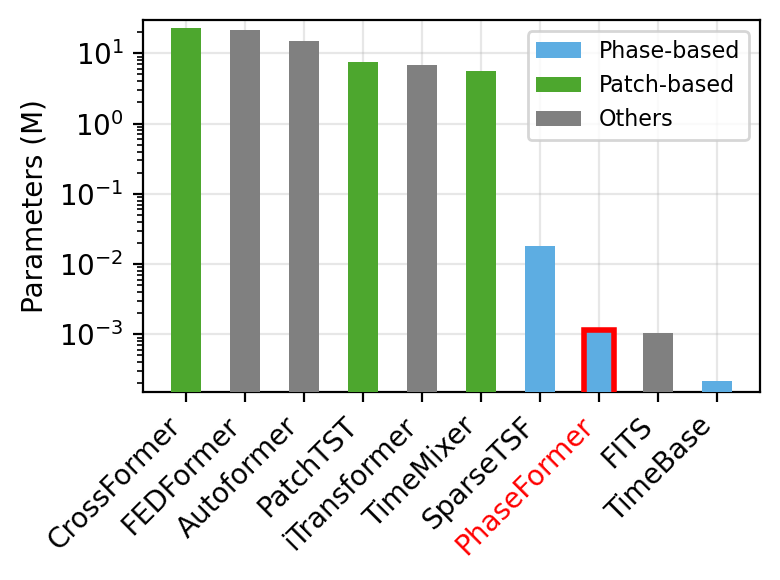
\includegraphics[width=\linewidth]{figures/params_traffic.png}
        \caption{Params on Traffic}
        \label{fig:traffic_params}
    \end{subfigure}
    % 子图3 - Electricity FLOPs
    \begin{subfigure}{0.24\textwidth}
        \centering
        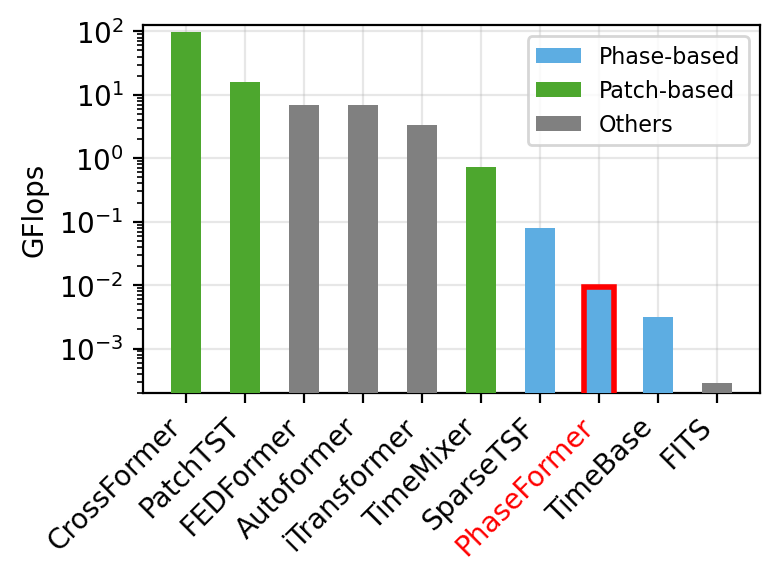
\includegraphics[width=\linewidth]{figures/flops_electricity.png}
        \caption{FLOPs on Electricity}
        \label{fig:electricity_flops}
    \end{subfigure}
    % 子图4 - Electricity Params
    \begin{subfigure}{0.24\textwidth}
        \centering
        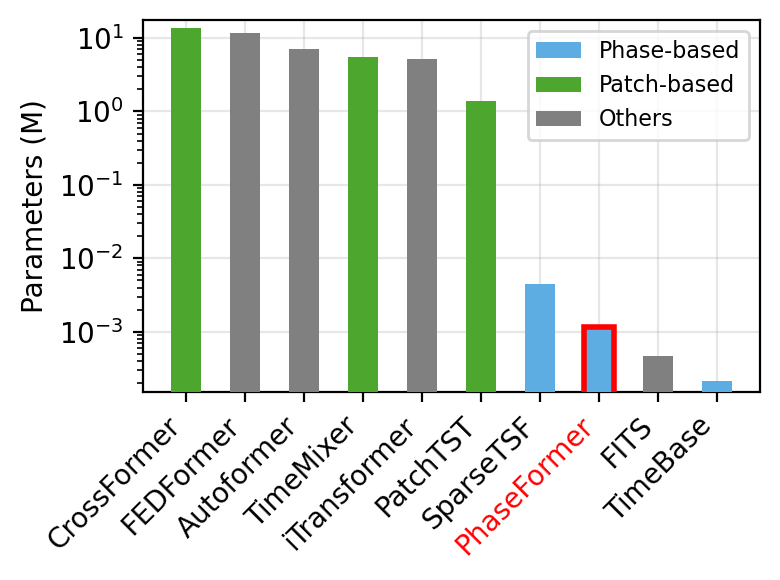
\includegraphics[width=\linewidth]{figures/params_electricity.png}
        \caption{Params on Electricity}
        \label{fig:electricity_params}
    \end{subfigure}
    \caption{
    Comparison of FLOPs and parameter counts across models on the Traffic and Electricity\revised{, using an input length of 720 steps and predicting 96 future steps}.
    Patch-based models are shown in green, phase-based models in blue, and other models in gray.
    }
    \label{fig:flops_params_visualization}
\end{figure*}


We evaluate the predictive accuracy of \sysname and the baseline methods on seven datasets. 
\tabref{tab:main_results} reports the average prediction errors across four forecasting horizons, with detailed results provided in \blue{the electronic supplement}.
\blue{Overall, \sysname attains the best average MSE on six of the seven datasets, with the clearest margins on the two large sensor networks: on Electricity it reduces the MSE by 3.0\% relative to the runner-up, iTransformer, and on the largest dataset, Traffic, by 2.0\% relative to PatchTST and by 7.7\% relative to TimeBase, underscoring its robustness on large-scale and heterogeneous data.}
\blue{The only exception is ETTh2, where FITS leads (0.334) and \sysname is within 0.002 of the second-best MSE (PatchTST, 0.344) and third in MAE.}
A closer examination reveals that patch-based baselines, including PatchTST, Crossformer, and TimeMixer, exhibit performance degradation on \blue{Electricity}.
\blue{The electronic supplement adds CycleNet to the comparison: on Electricity it attains a lower dataset average than both \sysname and \sysLA (0.157 against 0.160 and 0.159 in the full per-horizon tables of the supplement). We position this as a point on the efficiency trade-off rather than a like-for-like gap: CycleNet carries 472K parameters on Electricity and 563K on Traffic against the 1.16K of \sysname on both --- several hundred times more, a cost that grows with the number of channels through its learnable per-channel recurrent cycles (see the per-model parameter and FLOPs comparison in the electronic supplement).}

\blue{
\fakeparagraph{Results of \sysLA}
Table~\ref{tab:main_results} adds \sysLA, averaged over three seeds; per-horizon results with standard deviations are in Table~\ref{tab:la_full}. Against \sysname (conference), \sysLA improves the MSE on five of the seven dataset averages, by up to 1.6\% (Weather), and on 17 of the 28 settings; the MAE improves on 12 settings and four dataset averages (all comparisons on unrounded averages). These gains are conservative: the shared training protocol of the extension places \sysname (retrained) above its conference error on every dataset. Against \sysname (retrained), \sysLA improves the MSE on ETTh2, ETTm2 and Weather at every horizon by more than one seed standard deviation (Table~\ref{tab:la_full}), and on ETTm1 and Traffic the two models match: \sysname (retrained) averages 0.352 and 0.392 there, the \sysLA row 0.351 and 0.392. Section~\ref{sec:exp_theory} shows that ETTh2, ETTm2 and Weather are where the level envelope binds, and Section~\ref{sec:exp_ladder} attributes the gains to the two components under one protocol.
}

\subsection{\blue{Efficiency}}
\label{sec:exp_efficiency}

We evaluate the computational overhead of all models, with detailed results in \blue{the electronic supplement}.
\figref{fig:flops_params_visualization} shows the FLOPs and the number of parameters of all tested models on the Electricity and Traffic.
Overall, phase-based models incur lower overhead than patch-based ones.
On the Traffic dataset, \sysname achieves a FLOPs reduction of about 99.99\% over PatchTST and Crossformer.
Beyond patch-based baselines, it also outperforms other phase-based models like SparseTSF, consistently delivering high efficiency.
This stems from the \blue{stability} of phase tokens over time (\secref{sec:mot_stability}), making them inherently more efficient to process. 
Taken together with the previous accuracy evaluations, these results \blue{show} that \sysname provides an efficient yet effective solution, delivering superior performance on complex datasets.
\blue{The extension keeps this efficiency profile. Over \sysname, the level branch and the modulation of \sysLA add between 119 and 679 parameters in all 28 settings of the main-table configuration. The fusion gates add two parameters in total when they are shared and two per channel otherwise (1{,}724 on Traffic); they are the only component of the extension whose size grows with the number of sensors. Including them, the extension adds at most about 2.1K parameters, the largest increment being on Traffic (Section~\ref{sec:complexity} and Appendix~\ref{app:la_config}). Its added computation is linear in the input length and is dominated by the cost of the backbone.}
\blue{Measured on a single A800 GPU (fp32, batch 32, $L{=}720$), the extension adds between $0.09\%$ and $0.23\%$ to the FLOPs of the \sysname backbone on Traffic and Electricity, and between $3.9\%$ and $10.5\%$ to its latency: the added operations --- gates, fusions and pooling --- are element-wise and therefore memory-bound rather than compute-bound. The ratio falls as the backbone grows; on the smallest backbone (ETTh2-720, 718 parameters) the same absolute overhead amounts to about $37\%$ of its FLOPs and $71\%$ of its latency, the forward pass remaining below $2$\,ms.}

\subsection{\blue{Analysis of \sysname}}
\label{sec:exp_ablation}

\subsubsection{\blue{Ablation Studies}}

\fakeparagraph{Varying the Number of Routers}
We systematically evaluate the impact of different number of routers $M$ on model performance, with results summarized in \figref{fig:router_number_visualization}.
The experiments indicate that across three datasets, the model’s prediction error generally decreases as the number of routers $M$ increases, before eventually stabilizing or slightly rising.
It is worth noting that the best performance is usually achieved when $M \in \{4,8\}$, which is much smaller compared to the actual number of phase tokens, $L_{\text{phase}} = 24$.
This observation indicates that the phase token spans an inherently low-dimensional space, so only a small number of routers is sufficient to effectively capture and represent its underlying structure\blue{, in line with Insight~2 (Section~\ref{sec:mot_stability}), by which two dimensions explain over 90\% of the variance of phase tokens}.
More detailed results are provided in \blue{the electronic supplement}.

\begin{figure*}[t]
    \centering
    % 子图1
    \begin{subfigure}{0.32\textwidth}
        \centering
        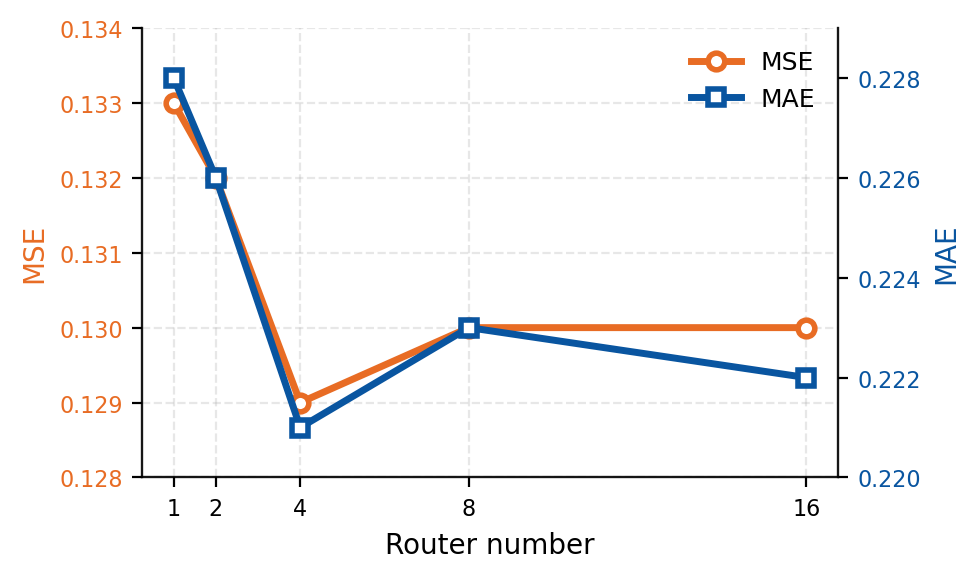
\includegraphics[width=\linewidth]{figures/router_number_effect_electricity_lines.png}
        \caption{Electricity}
        \label{fig:electricity}
    \end{subfigure}
    % 子图2
    \begin{subfigure}{0.32\textwidth}
        \centering
        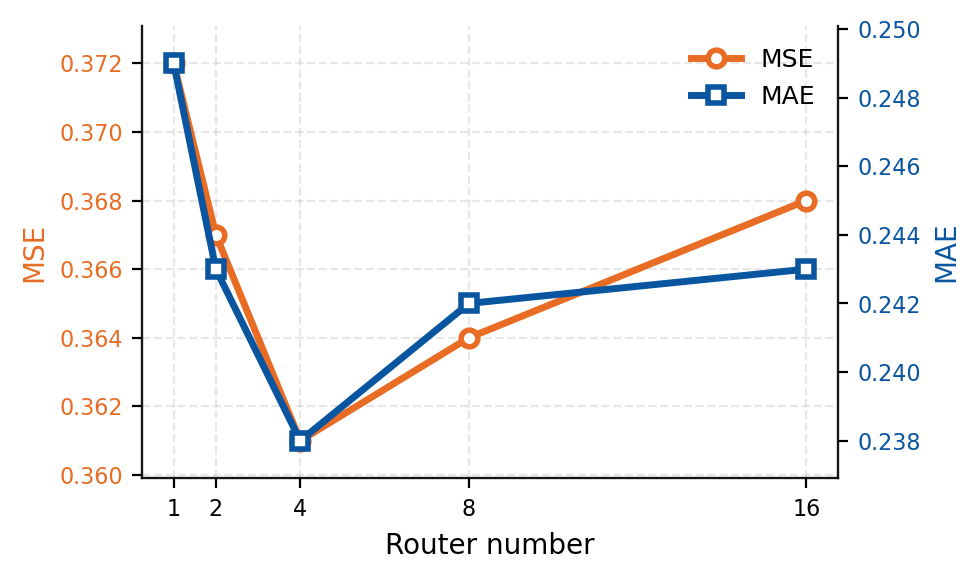
\includegraphics[width=\linewidth]{figures/router_number_effect_traffic_lines.png}
        \caption{Traffic}
        \label{fig:traffic}
    \end{subfigure}
    % 子图3
    \begin{subfigure}{0.32\textwidth}
        \centering
        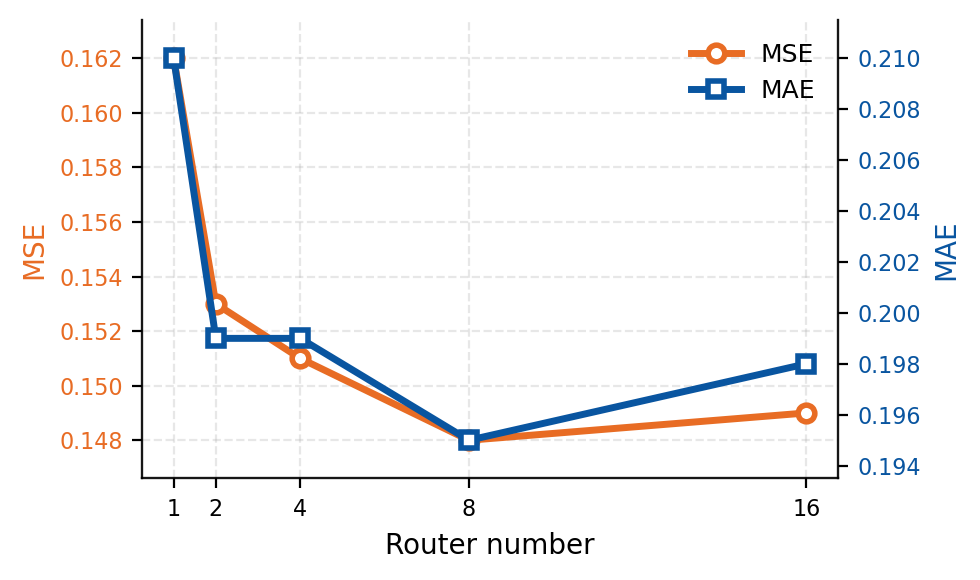
\includegraphics[width=\linewidth]{figures/router_number_effect_weather_lines.png}
        \caption{Weather}
        \label{fig:Weather}
    \end{subfigure}
    
    \caption{Effect of varying the number of routers $M$ on forecasting performance on three datasets.}
    \label{fig:router_number_visualization}
\end{figure*}



\begin{table*}[t]
\centering
\caption{Cross-Phase Routing layer ablation. Each cell reports MSE, MAE, and FLOPs. Lower is better for all metrics. FLOPs are reported in millions (MFLOPs). The best results are highlighted with \best{Bold}, and the second-best results with \second{Underlined}.}
\label{tab:ablation_phase}
\footnotesize
\begin{tabular}{c|ccc|ccc|ccc|ccc}
\hline
\multirow{2}{*}{Dataset}
& \multicolumn{3}{c|}{\textbf{\sysname}} 
& \multicolumn{3}{c|}{\textbf{w/ FullAttention}} 
& \multicolumn{3}{c|}{\textbf{w/ LinearMixing}} 
& \multicolumn{3}{c}{\textbf{w/o Routing}} \\
\cline{2-13}
& MSE & MAE & FLOPs 
& MSE & MAE & FLOPs 
& MSE & MAE & FLOPs 
& MSE & MAE & FLOPs \\
\hline
Weather 
& \best{0.1503} & \best{0.1971} & 3.119 
& \second{0.1527} & \second{0.2005} & 3.202 
& 0.1700 & 0.2226 & \second{0.920} 
& 0.1907 & 0.2406 & \best{0.783} \\
\hline
Electricity 
& \best{0.1290} & \best{0.2209} & 42.213 
& \second{0.1295} & \second{0.2217} & 48.951 
& 0.1403 & 0.2334 & \second{14.068} 
& 0.1423 & 0.2365 & \best{11.972 } \\
\hline
Traffic     
& \best{0.3721} & \best{0.2475} & 113.356 
& \second{0.3791} & \second{0.2513} & 131.452 
& 0.3842 & 0.2532 & \second{37.776}
& 0.3892 & 0.2584 & \best{32.149}  \\
\hline
\end{tabular}
\end{table*}




\fakeparagraph{Effectiveness of Cross-Phase Routing} 
To assess the contribution of the cross-phase routing layer, we compare four variants of the model: 
\textbf{\sysname}, which adopts the original cross-phase routing layer; 
\textbf{w/ FullAttention}, which substitutes the cross-phase routing layer with a full attention mechanism;
\textbf{w/ LinearMixing}, which replaces the cross-phase routing layer with a linear layer; and 
\textbf{w/o Routing}, which directly projects each phase into its own future.
All other experimental settings are kept identical across these variants. 

As summarized in \tabref{tab:ablation_phase}, \sysname consistently outperforms \textbf{w/ LinearMixing} and \textbf{w/o Routing}, indicating that explicit cross-phase routing is crucial for modeling periodic dynamics. Moreover, \sysname not only incurs less \blue{computation}, but also achieves lower prediction error than \textbf{w/ FullAttention}, showing that the routing layer is both efficient and effective. We attribute these gains to operating in a low-dimensional phase token space, which concentrates informative interactions and reduces cost.

\revised{
\subsubsection{Sensitivity Analysis of Phase Length Choices}
\label{sec:phase_length}

\begin{table}[t]
\centering
\begin{tabular}{ccc}
\hline
\textbf{Phase Length} & \textbf{MSE} & \textbf{MAE} \\
\hline
24 & 0.3619 & 0.2384 \\
12 & 0.3960 & 0.2765 \\
8  & 0.4032 & 0.2801 \\
28 & 0.4063 & 0.2753 \\
21 & 0.4184 & 0.2970 \\
\hline
\end{tabular}
\caption{Comparison of forecasting performance under different phase lengths on the Traffic dataset (\blue{$L=720$, $H=96$}).}
\label{tab:phase_length}
\end{table}
\sysname automatically determines the phase length through frequency-domain analysis (see \blue{the electronic supplement}), extracting salient periodic components directly from the data.
To assess its sensitivity to phase length, we conduct experiments on the Traffic dataset. Its frequency spectrum contains several clear periodic components (see \figref{fig:spectrum_traffic}). Based on spectral amplitudes, we select the top five candidate phase lengths and run \sysname for forecasting. The results are shown in \tabref{tab:phase_length}.

\begin{figure}[t]
    \centering
    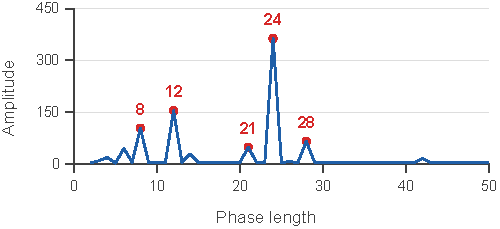
\includegraphics[width=\linewidth]{figures/spectrum_traffic.pdf}
    \caption{The spectrum calculated on the Traffic dataset. The top-5 phase length is 24, 12, 8, 28, 21.}
    \label{fig:spectrum_traffic}
\end{figure}

The experiments show that the model performs best when the phase length is 24, corresponding to the dominant spectral component. \blue{The errors of the five candidates increase exactly in the order of their spectral amplitudes (\figref{fig:spectrum_traffic}), so the strongest spectral component is also the most accurate phase length.}
These findings demonstrate that \sysname effectively captures the dataset’s primary periodic structure.
}

\subsubsection{Case Study}
\label{sec:exp_case}
We select one sample from Traffic dataset, comprising an input sequence of length 720 and an output sequence of length 96 (816 time steps in total). 
The input sequence is fed into \sysname, and we record the attention-weight matrices at the first cross-phase routing layer during both aggregation (Phase$\rightarrow$Router) and distribution (Router$\rightarrow$Phase).
As shown in \figref{fig:sender} and \figref{fig:receiver}, both attention patterns exhibit clear local similarity: adjacent phases tend to be assigned to the same routers and to receive attention from similar routers.
This indicates that the routing mechanism captures temporally consistent phase relationships. 
Meanwhile, the attention weights reveal that certain phases share similar attentive patterns.
To analyze this further, we focus on three phases with distinct attentive patterns and \blue{visualize} them in \figref{fig:traffic_data_visualization}.
These phases display different temporal behaviors: Phase 5 remains relatively stable over long horizons, whereas Phase 9 and Phase 1 both exhibit a pronounced 7-day periodicity but with opposite trends.
The differing patterns of these phase tokens suggest that the router structure not only distinguishes among phase tokens but also effectively models their periodicity and trend characteristics.


\begin{figure*}[t] 
  \centering
  \begin{subfigure}{0.24\linewidth}
    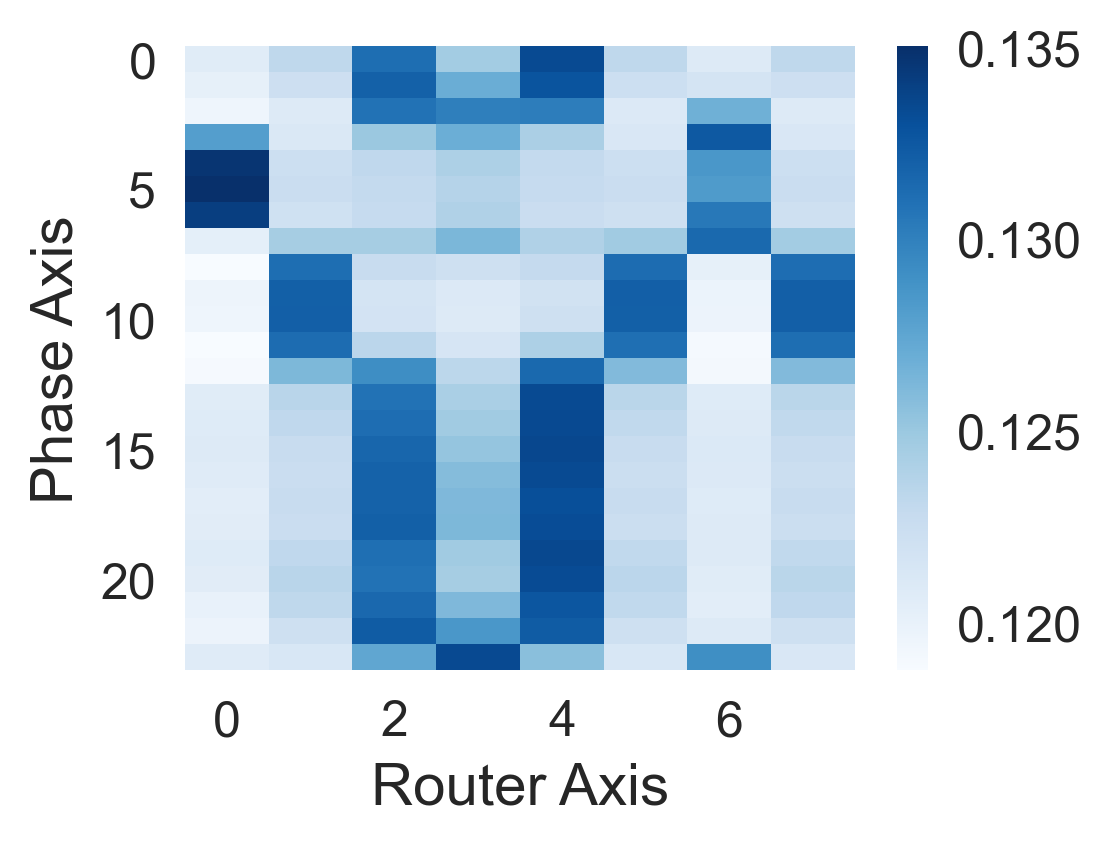
\includegraphics[width=\linewidth]{figures/attention_layer_0_sender_var4.png}
    \caption{Aggregation Weights}
    \label{fig:sender}
  \end{subfigure}%
  \hfill
  \begin{subfigure}{0.24\linewidth}
    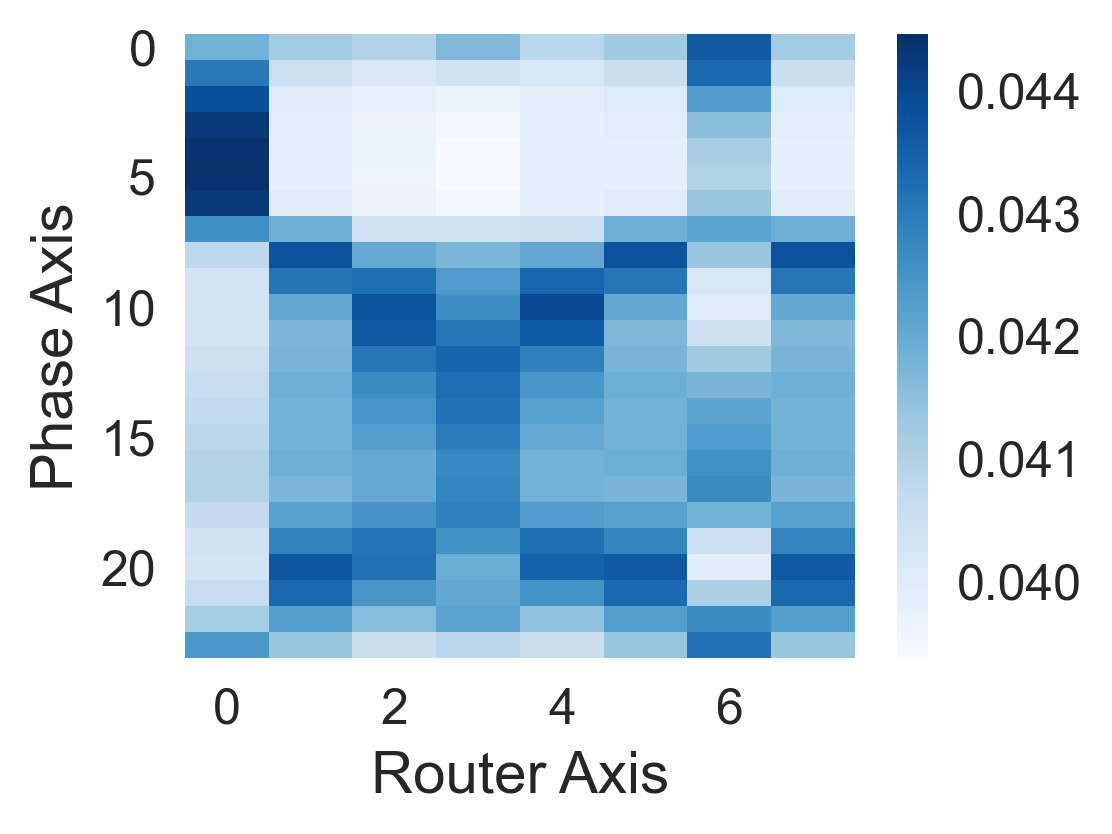
\includegraphics[width=\linewidth]{figures/attention_layer_0_receiver_var4.png}
    \caption{Distribution Weights}
    \label{fig:receiver}
  \end{subfigure}
  \hfill
  \begin{subfigure}{0.48\linewidth}
    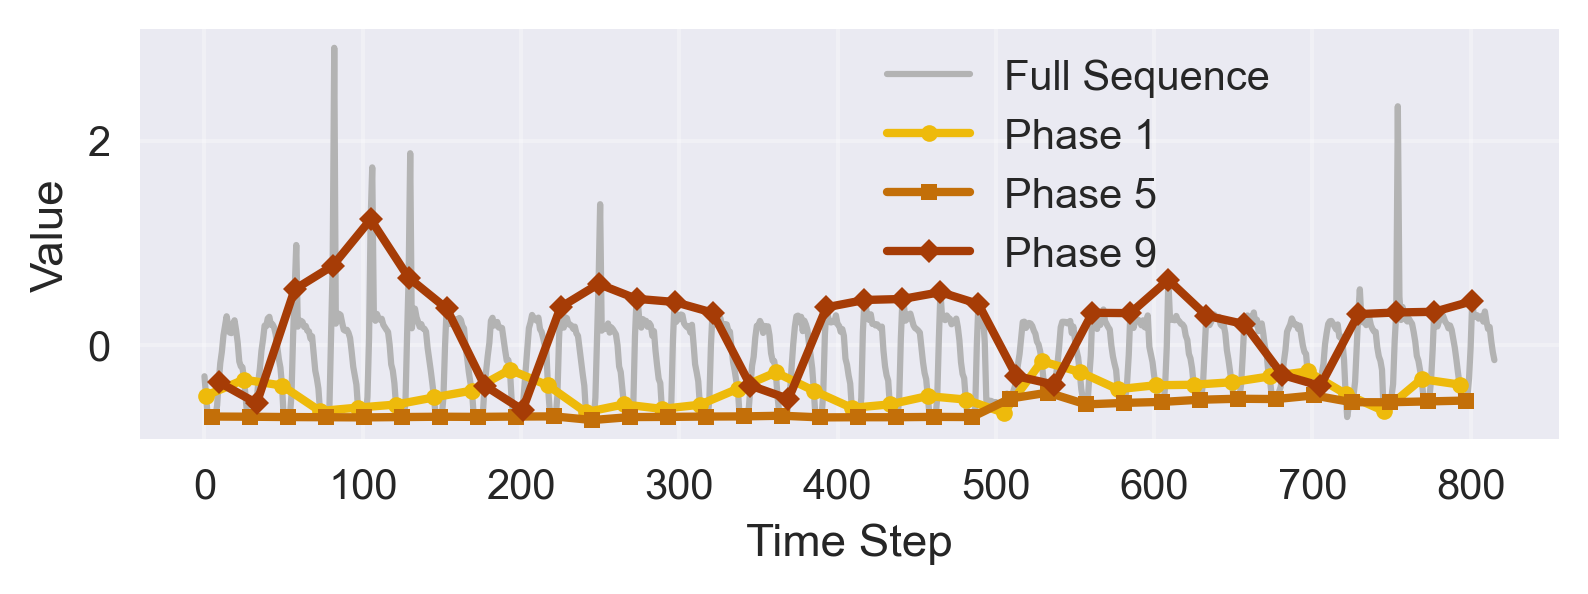
\includegraphics[width=\linewidth]{figures/sequence_with_phase_curves_sample_0_feature_0.png}
    \caption{Visualization of three selected phase tokens}
    \label{fig:traffic_data_visualization}
  \end{subfigure}%
  \caption{Case study on a sample from the Traffic dataset. 
  (a) Attention weight matrix during Phase-to-Router aggregation. 
  (b) Attention weight matrix during Router-to-Phase distribution. 
  Both matrices capture the association between 8 routers and 24 input phases. 
  (c) Visualization of three representative phases (1, 5, and 9), each represents a distinct attentive pattern with routers.} 
  \label{fig:case_study_wrap_all}
\end{figure*}


\blue{
\subsection{Validating the Theory}
\label{sec:exp_theory}

Section~\ref{sec:theory} argues in four steps. Step~(i), that \sysname can represent level drift, is established by construction (Proposition~\ref{prop:capability}). Steps~(ii)--(iv) make predictions that can be checked on trained checkpoints: that the envelopes hold on every checkpoint and bind where the demands of the data exceed them, and that the branch takes over the level there (Section~\ref{sec:exp_envelopes}); that the modulation preserves the cycle means and reads the level (Section~\ref{sec:exp_mechanism}); and that a few fixed profiles suffice for the level branch (Section~\ref{sec:exp_capacity}). Section~\ref{sec:exp_ladder} then measures what each component gains.

\subsubsection{Envelopes and Level Hand-over on Trained Checkpoints}
\label{sec:exp_envelopes}

The constants of Theorems~\ref{thm:level_envelope} and~\ref{thm:amplitude} are functions of the weights, so they can be read from every trained checkpoint, and the demands are functions of the data. Table~\ref{tab:envelope} reports both for the \sysLA checkpoints (averaged over the four horizons), together with the level demand $\Lambda$ and the amplitude demand $\Omega$ of every test window.

\begin{table}[t]
\blue{
\centering
\caption{Envelopes of the phase path on trained \sysLA checkpoints (protocol configuration; averages over the horizons; modulation switched off). $C_1$, $B_\varphi$: half-width of the level envelope and amplitude envelope, read from the weights; $g_s$: shape gate; outside $\mathcal I_\varphi$: share of test windows whose level demand $\Lambda$ lies outside the level envelope; floor/MSE: error floor~\equref{eq:level_floor} as a share of the test MSE; $\Omega$ over env.: share of windows whose amplitude demand exceeds $(1-g_s)B_\varphi$.}
\label{tab:envelope}
\footnotesize
\setlength{\tabcolsep}{2.6pt}
\begin{tabular}{lcccccc}
\toprule
Dataset & $C_1$ & $B_\varphi$ & $g_s$ & outside $\mathcal I_\varphi$ & floor/MSE & $\Omega$ over env. \\
\midrule
ETTh1 & 1.35 & 1.37 & 0.23 & 2.5\% & 0.08\% & 14.8\% \\
ETTh2 & 1.07 & 1.08 & 0.25 & 19.4\% & 5.0\% & 31.8\% \\
ETTm1 & 1.86 & 1.99 & 0.35 & 3.5\% & 0.27\% & 2.2\% \\
ETTm2 & 1.39 & 1.47 & 0.26 & 12.5\% & 10.6\% & 5.7\% \\
Weather & 1.41 & 1.61 & 0.68 & 20.7\% & 11.6\% & 27.6\% \\
Electricity & 3.80 & 3.81 & 0.27 & 0.1\% & 0.5\% & 0.2\% \\
Traffic & 5.23 & 5.25 & 0.21 & 0.0\% & 0.0\% & 0.0\% \\
\bottomrule
\end{tabular}
}
\end{table}

Three observations. First, the level envelope holds exactly as stated: across all 84 checkpoints (28 settings, three seeds), the measured levels of the phase forecast never leave $\mathcal I_\varphi$, the largest observed value of $|\lev(F)-c_0|/C_1$ being $0.74$, so the floors below are conservative. Second, where the envelope binds, it binds in the way the theory predicts. On ETTh2, Weather and ETTm2, between 12\% and 21\% of test windows have a level demand outside the interval, the floor accounts for 5.0\% to 11.6\% of the test MSE, and on ETTh2 and Weather both the share of out-of-envelope windows and the tightness of the interval grow with the horizon (ETTh2: $C_1$ from 1.27 to 0.85 and the outside share from 15\% to 27\% between $H=96$ and $H=720$; Weather: 1.86 to 0.96 and 10\% to 34\%). On the two sensor networks the trained checkpoints developed wide envelopes that almost no test window escapes. Their half-widths, $C_1$ between 3.8 and 5.2, stay below the 5.39 needed to track the level of the last cycle uniformly (Section~\ref{sec:theory_level}), but the level demands of the test windows are smaller, and the floor is at most 0.5\% of the test MSE. The envelopes thus force almost no loss on the phase path there, and Section~\ref{sec:exp_ladder} shows that, under one protocol, the extension changes the error on these datasets by less than 1\%.

Third, the hand-over follows the envelope. The level gate stays near its initialization value on every dataset ($g_\ell$ between 0.20 and 0.26 on average), but what the branch does with its share depends on whether the envelope binds: the correlation between the branch's level and the window's level demand is between $0.40$ and $0.44$ on the four ETT datasets, whose envelopes are narrow ($C_1\le1.86$), and $0.03$ and $-0.01$ on Electricity and Traffic, whose envelopes are wide. The branch tracks the level where the phase path cannot, as Theorem~\ref{thm:complement}(b) predicts.

\begin{table*}[t]
\blue{
\centering
\caption{Ablation ladder, test MSE/MAE averaged over the four horizons and three seeds (protocol configuration, Section~\ref{sec:ext_setup}). \sysname (retrained) is the backbone retrained under this protocol; \sysLA (mod.\ off) is \sysLA with the modulation disabled on the trained checkpoint.}
\label{tab:ladder}
\footnotesize
\setlength{\tabcolsep}{6pt}
\begin{tabular}{lcccccccc}
\toprule
Dataset & \multicolumn{2}{c}{\begin{tabular}[c]{@{}c@{}}\sysname\\(retrained)\end{tabular}} & \multicolumn{2}{c}{\sysL} & \multicolumn{2}{c}{\sysLA} & \multicolumn{2}{c}{\begin{tabular}[c]{@{}c@{}}\sysLA\\(mod.\ off)\end{tabular}} \\
\cmidrule(lr){2-3}\cmidrule(lr){4-5}\cmidrule(lr){6-7}\cmidrule(lr){8-9}
 & MSE & MAE & MSE & MAE & MSE & MAE & MSE & MAE \\
\midrule
ETTh1 & 0.408 & 0.419 & 0.412 & 0.425 & \textbf{0.405} & \textbf{0.421} & 0.414 & 0.429 \\
ETTh2 & 0.354 & 0.396 & \textbf{0.347} & \textbf{0.393} & 0.348 & \textbf{0.393} & 0.352 & 0.396 \\
ETTm1 & \textbf{0.352} & \textbf{0.377} & 0.354 & 0.380 & 0.353 & 0.380 & 0.355 & 0.381 \\
ETTm2 & 0.258 & 0.319 & \textbf{0.253} & \textbf{0.315} & \textbf{0.253} & \textbf{0.315} & 0.257 & 0.318 \\
Weather & 0.227 & 0.262 & 0.221 & 0.257 & \textbf{0.220} & \textbf{0.257} & 0.220 & 0.257 \\
Electricity & 0.161 & 0.251 & \textbf{0.160} & \textbf{0.251} & \textbf{0.160} & \textbf{0.251} & 0.162 & 0.254 \\
Traffic & \textbf{0.392} & \textbf{0.248} & 0.395 & 0.251 & 0.393 & 0.252 & 0.400 & 0.256 \\
\bottomrule
\end{tabular}
}
\end{table*}

\subsubsection{Mechanism of the Modulation}
\label{sec:exp_mechanism}

\fakeparagraph{Synthetic multiplicative series}
We first test Theorem~\ref{thm:amplitude} where the ground truth is known. We generate seven-channel series from \equref{eq:mult_model} with a random-walk level, a sinusoidal daily profile and coupling $\alpha\in\{0,0.25,0.5\}$, and train \sysL and \sysLA from the same initialization (two seeds, 30 epochs). Without coupling ($\alpha=0$), the modulation has nothing to carry and the two models are indistinguishable: \sysLA changes the validation MSE by $-0.28\%$. With coupling, \sysLA reduces the validation MSE by $3.3\%$ at $\alpha=0.25$ and by $4.8\%$ at $\alpha=0.5$, and it does so for both seeds. The gain appears exactly when the data contain level-dependent amplitude and grows with the coupling, as the form of the demand in Theorem~\ref{thm:amplitude}(b) and the construction of Proposition~\ref{prop:modulation}(b) imply.

\fakeparagraph{Cycle-mean invariance}
Proposition~\ref{prop:modulation}(a) is an exact identity, so we verify it on every trained \sysLA checkpoint. Switching the modulation off and on, in double precision, changes every future cycle mean of the phase forecast by at most $8.9\times10^{-16}$ in absolute value, against a tolerance of $7\times10^{-9}$ relative to the forecast scale, while it changes individual phase forecasts by up to $1.8$ window standard deviations. All 84 checkpoints (28 settings, three seeds) pass.

\fakeparagraph{What drives the modulation}
Proposition~\ref{prop:modulation}(b) predicts that the modulation reads the level: its construction in Appendix~\ref{app:proofs}, $q=\alpha_w\one_d\,\xi^\top t$ with $\xi^\top t$ the branch's level forecast, scales the phase amplitude by the factor $1+\alpha_w\hat\Lambda$. The trained checkpoints bear this out, most clearly at $H=96$, and where they read the level less, the modulation acts as a static per-channel amplitude correction, which a uniform part of $q$ provides (Section~\ref{sec:theory_amplitude}). We correlate, per channel, the component of $q$ along $\one_d$ with the window's level demand $\Lambda$; pooling channels would mix the level-driven part of $q$ with its channel-dependent static scale. At $H=96$, the mean per-channel correlation is $0.46$ on Weather (86\% of channels), $0.30$ on Electricity, where all 166 significant channels share one sign, and $0.54$ on ETTh2, with every channel above $0.3$; averaged over the horizons it is between $0.12$ and $0.37$ on the seven datasets. The sign of the learned coupling is consistent within each setting --- the significant channels of Weather-$96$ share the sign opposite to that of Electricity-$96$ --- which the construction allows, since $\alpha_w$ is learned.

On ETTm1-$96$ and ETTm2-$96$ the correlation is lower ($0.27$ and $0.02$): there the modulation acts mostly as the static correction. On ETTh2 and Weather the correlation is lower at longer horizons, where the persistent-level idealization of Theorem~\ref{thm:amplitude}(b) is less accurate. Two further observations agree with the construction: $q$ is only weakly correlated with the amplitude demand $\Omega$ itself (mean per-channel correlation below $0.20$ everywhere), so it follows the level rather than the amplitude; and the static part of $q$ is a per-channel amplitude correction whose removal accounts for the degradation of the modulation-off column of Table~\ref{tab:ladder} on six of the seven datasets.

\subsubsection{Capacity of the Level Branch}
\label{sec:exp_capacity}

Theorem~\ref{thm:complement}(a) predicts that, under standard seasonal models, the level the phase path misses enters through a few fixed horizon profiles, so a branch whose profiles are fixed in advance should lose nothing against one that learns them. The selection experiment of Section~\ref{sec:ext_setup} provides a direct check. At the same rank, the three decoders differ widely in parameter count: the learned decoders have $93+4H$ and $273+4H$ parameters, up to 3{,}153 at $H=720$, whereas the fixed profiles have 105 parameters. Yet their setting-normalized validation errors, averaged over seven datasets and both gate variants, differ by only 0.13\%: 1.0102 for the decoder on 90 pooled values, 1.0107 for the decoder on 30 pooled values and 1.0115 for the fixed profiles, relative to the best variant of each setting. The fixed profiles sit within the 0.5\% tie of the best decoder and are preferred as the smallest. A branch restricted to the span of the displacement, tilt and curvature profiles therefore loses essentially nothing against branches that can learn arbitrary horizon profiles, as Theorem~\ref{thm:complement}(a) predicts, and these three profiles suffice. The protocol configuration keeps the fixed profiles on every setting; the per-setting search of the main-table configuration, which also weighs small per-setting differences, selects a learned decoder on ETTm1-720 and on three of the four horizons of ETTm2 (Appendix~\ref{app:la_config}).
}

\blue{
\subsection{From \sysname to \sysLA}
\label{sec:exp_ladder}
Table~\ref{tab:ladder} adds the components one at a time, on all 28 settings with three seeds, under the protocol configuration of Section~\ref{sec:ext_setup}. Its first column is \sysname (retrained), so the ladder isolates the components; its last column disables the modulation on the trained \sysLA checkpoint.



The two steps contribute differently, and the difference follows the theory. The level branch gains exactly where the level envelope binds (Table~\ref{tab:envelope}): on ETTh2, ETTm2 and Weather, where between 12\% and 21\% of the test windows lie outside the envelope, it improves the MSE by 2.0\%, 1.8\% and 2.7\%, while on the four datasets where at most 3.5\% lie outside, it changes the error by at most 1.0\%. Over all settings, \sysL improves on \sysname (retrained) in 17 of the 28. The modulation adds what the level branch cannot. ETTh1 is the one dataset whose amplitude envelope binds (14.8\% of the windows) while its level envelope barely does (2.5\%); there the branch alone costs 1.0\%, the modulation carries the recovery, and \sysLA ends 0.7\% below \sysname (retrained). Disabling the modulation on the trained checkpoint gives back the entire difference (0.414 against 0.405). Across all 28 settings, the modulation improves its own checkpoint in 27 cases, and \sysLA improves on \sysname (retrained) in 17.

Under one protocol, \sysLA thus improves five of the seven dataset averages, by between 0.4\% and 3.3\% (computed on unrounded averages), and stays within 0.3\% of \sysname (retrained) on ETTm1 and Traffic, at a parameter cost of about 130--170, excluding the fusion gates, in the protocol configuration. This matches Section~\ref{sec:theory_design}: the extension addresses the changes across cycles, and it gains most where Section~\ref{sec:exp_envelopes} shows them to bind. On ETTh2 and ETTm2, the two least coupled benchmarks (Section~\ref{sec:mot_changes}), the modulation adds nothing over \sysL (0.348 against 0.347, and 0.253 on both): with coupling this weak, the 31.8\% of ETTh2 windows over the amplitude envelope owe their excess to the windows' own shape $\Omega_0$ rather than to the level. On Traffic, the most coupled benchmark, the modulation improves its own checkpoint (0.393 against 0.400 with the modulation off) although no window exceeds the envelope; the gain combines the static per-channel correction of $q$ (Section~\ref{sec:exp_mechanism}) with a level-dependent part, which the stratification below brings out.

\fakeparagraph{Where the gain occurs}
If the modulation carries the level-dependent amplitude, the per-window gains of \sysLA over \sysL should grow with the level demand. Stratifying the per-window test gains by the quintiles of $|\Lambda|$ supports this. Across all 28 settings, the top quintile gains $0.002$ MSE more than the bottom one, and on 12 of the 17 settings where \sysLA improves on average, the mean gain of the top quintile exceeds that of the bottom one, with the strongest settings rising from bottom to top (Traffic-$96$: $+0.0002$ to $+0.0033$ across the quintiles; ETTh1-$192$: $-0.0033$ to $+0.0052$; Weather-$96$: $-0.0031$ to $+0.0080$). The modulation thus gains most on the windows whose level moves most.

\fakeparagraph{Summary}
\sysname attains the best average MSE on six of the seven benchmarks at a fraction of the cost of its baselines. On trained checkpoints, the level envelope of Section~\ref{sec:theory} holds on every checkpoint and binds on exactly the three datasets where the level branch gains most, the modulation preserves every cycle mean exactly and reads the level, and three fixed profiles suffice for the level branch. Together, the two components let \sysLA improve five of the seven dataset averages under one protocol at a cost of about 130--170 parameters, excluding the fusion gates, while costing at most 0.3\% on the two datasets they do not improve.
}
